\section{Teoría de los mercados eficientes}
% explicación muy densa, revisitar y rescribir
Las finanzas, en parte, son una herramienta para enfrentarse a la incertidumbre. Al igual como puede ser el ahorro o un seguro las carteras de activos buscan minimizar el riesgo que enfrenta un inversor al buscar cierto retorno esperado. 

En 1952 \textbf{Harry Markowitz}\marginnote{\textbf{Harry Markowitz (1927-2023):} Economista estadounidense, premio nobel del 1990 gracias su aporte a la economía financiera.} presentó un modelo de formación de carteras en el cual inversores racionales con información respecto a los activos en disposición formarían una cartera riesgo-eficiente que se ajuste a sus preferencias de aversión al riesgo. El modelo de Markowitz no es tan complejo y maneja conceptos ya bastante discutidos en capítulos anteriores, como pueden ser individuos aversos al riesgo, maximizadores de utilidad sujetos a restricciones.

Anteriormente graficabamos la función de utilidad de un individuo como una función cóncava en caso de que este sea averso al riesgo. Una extensión del análisis sería armar curvas de diferencia entre el retorno esperado de un proyecto y el riesgo que conllevaría tomarlo. Esto es, para determinado rendimiento cuánto riesgo está determinado asumir el inversor. 
% Falta hacer un gráfico comparando las curvas de indiferencia de aversos, neutros y amantes del riesgo
\begin{figure}[ht]
    \centering
    \caption{Curvas de indiferencia riesgo-retorno}
    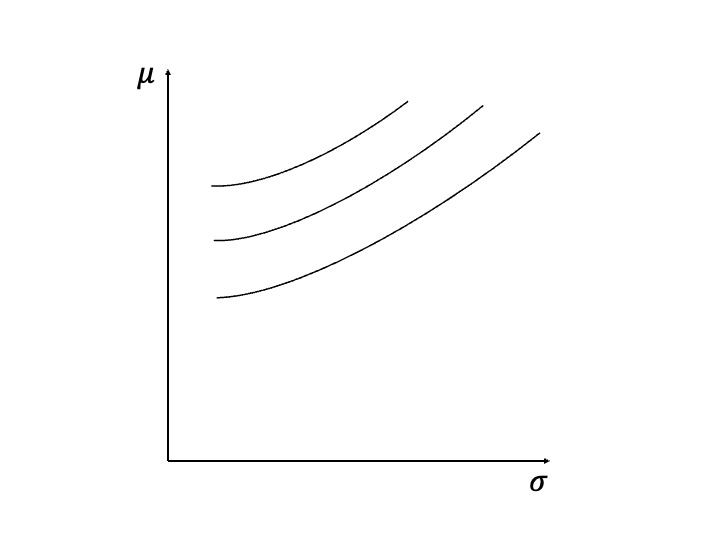
\includegraphics[width=10cm]{Figuras/Curvas de indiferencia riesgo-retorno.jpeg}
    \label{fig: Curvas de indiferencia riesgo-retorno}
\end{figure}
Los individuos preferirán un proyecto más riesgoso que otro siempre y cuando el rendimiento esperado sea suficiente o más para compensar la incertidumbre adicional. Las curvas de indiferencia (Figura \ref{fig: Curvas de indiferencia riesgo-retorno}) serán siempre convexas para todo individuo independiente si son aversos, neutros o amantes del riesgo. Sin embargo, mientras más aversos al riesgo sean más convexa será esta curva de indiferencia, dejándose ver que ante un mayor riesgo necesitan un incremento cada vez mayor de rendimiento esperado.

\subsection{Teoría de carteras, el problema financiero}

El problema de administración de \textbf{carteras}\marginnote{\textbf{Cartera de activos:} Una cartera o portafolio de activos hace referencia a una colección de distintos activos que se juntan en pos de diversificar riesgo.} hace referencia a la distribución y minimización del riesgo al buscar cierto retorno esperado. Las carteras son colecciones de activos los cuales tienen sus respectivos retornos y riesgos, cada activo puede estar más o menos presente en la cartera dependiendo de la composición de esta. 

El \textbf{precio} de una cartera en $t = 0$ puede ser descrito como la sumatoria del valor de los activos $A_i$ en dicho período.
\begin{equation}
    P_0 = \sum ^{I}_{i = 1} A_{i0}
\end{equation}
Mientras que el \textbf{retorno esperado}\marginnote{\textbf{Retorno esperado:} El retorno promedio de un activo o cartera de activos sujeto a incertidumbre y varianza.} que obtengamos de una cartera dependerá obviamente del retorno de cada activo, pero además del peso de dicho activo en la cartera. 
\begin{equation}
    r_p = \sum^{I}_{i = 1}\frac{A_{i0}}{P_0} r_{i0}
\end{equation}
Por otro lado, el riesgo\footnote{Con riesgo generalmente nos referimos a la desviación estándar del activo o portafolio.} de una cartera no se corresponde a simplemente la suma de las varianzas, esto ya que entra en juego las correlaciones de los activos entre sí. Es decir, no nos fijamos en como se comportan los activos por separado sino la combinación de dichos activos en un mismo portafolio. Veamos esto más en detalle:

Ahora mismo vamos a dejar de lado el tema riesgo-retorno para centrarnos en la minimización de riesgo, definiendo los puntos importantes que permiten que al juntar activos reduzcamos el riesgo del portafolio. Es necesario conocimientos elementales de estadística, los cuales se pueden encontrar en el anexo.

Para un portafolio de dos activos riesgosos $i$ con esperanza $\mu_i$ y varianza $\sigma^2_i$,
\begin{align*}
    X \sim (\mu_X,\sigma_X^2), \quad Y \sim(\mu_Y,\sigma_Y^2)
\end{align*}
El portafolio está compuesto por una fracción $0\leq a \leq 1$ de $X$ y por una fracción $0\leq b \leq 1$ de $Y$. Entonces podemos escribir la varianza del portafolio como $\mathbb{V}(aX + bY)$. Es decir, la suma de la varianza de los activos $X$ e $Y$ y de la covarianza entre los mismos. 
\begin{equation}
    \mathbb{V}(aX+bY) = a^2\sigma_X^2 + b^2\sigma_Y^2 + 2ab\text{Cov}_{XY} \label{eq: riesgo de portafolio suma}
\end{equation}
Como se puede observar la varianza del portafolio completo no es sólo la suma de las varianzas de los activos por separado sino también la interacción (covarianza) entre los mismos.

Es directo observar en \ref{eq: riesgo de portafolio suma} que si la covarianza entre los activos es positiva la varianza del portafolio será mayor que la suma de las varianzas. En este caso, se juntaron dos activos volátiles que juntos hacen una cartera aún más volátil, lo cúal a menos que presente rendimiento esperado tan alto que compense la incertidumbre, no valdría la pena. 

La idea del portafolio que estamos buscando en este momento es que reduzcamos el riesgo al que el inversor se enfrenta. Para esto se necesitan activos que juntos reduzcan el riesgo de portafolio, condición para esto es que sean independientes o que covarien negativamente. Obviamente si la covarianza en \ref{eq: riesgo de portafolio suma} es negativa el riesgo del portafolio bajará puesto que en caso de que a un activo le vaya mal lo más probable es que el otro la vaya bien.

Mostremos que aun cuando los activos son independientes el riesgo del portafolio baja. En caso de que $X$ e $Y$ fueran independientes implicaría que $\text{Cov}_{XY}= 0$. Asumiendo que tienen varianzas $\sigma_X^2 = \sigma^2_Y = 1$. Tendríamos que la desviación estándar del portafolio sería $\mathbb{SD}(aX + bY) = \sqrt{a^2 + b^2}$, mientras que la sumatoria de las desviaciones de los activos por separado serían $a+b$. Como se puede ver en la figura \ref{fig: Diversificación del riesgo con dos activos} por teorema de Pitágoras, siempre se cumplirá que $\sqrt{a^2 + b^2} < a+b$.

\begin{figure}[ht]
    \centering
    \caption{El riesgo de un portafolio será menor que la suma de los riesgos de los activos que lo componen}
    \includegraphics[width=11cm]{Figuras/Riesgo de un portafolio y reducción de riesgo.jpeg}
    \label{fig: Diversificación del riesgo con dos activos}
\end{figure}

Reduciremos riesgo juntando activos siempre y cuando sean independientes o covaríen negativamente. En el caso anterior fueron dos activos, pero generalizemos para $N$. Formando una cartera de $N$ activos $X_i$ de igual varianza con pesos iguales cada uno, podemos escribir la varianza de la cartera de esta manera,
\begin{align*}
    \mathbb{V} \left(\sum_{i =1}^{N} \frac{X_i}{N} \right) = \frac{1}{N^2}\mathbb{V} \left(\sum_{i = 1}^N X_i \right) = \frac{N\sigma^2}{N^2} = \frac{\sigma^2 X}{N}
\end{align*}
Mientras más activos independientes conformen la cartera en partes iguales se diversifica el riesgo por lo que disminuye la varianza de la cartera.
\begin{equation}
    \lim_{N \to \infty} \frac{\sigma^2 X}{N} = 0
\end{equation}
Ahora finalmente definamos finalmente la varianza de una cartera de activos $i$ donde cada uno pesa una fracción $w_i$ en la cartera y tienen una varianza $\sigma^2_i$. 
\begin{equation}
    \sigma_{P_0}^2 = \sum_{i = 1}^I w_{i0}^2\sigma_i^2 + \sum^I_{i = 1}\sum^I_{i \neq j} w_{i0}w_{j0}\text{Cov}_{ij}
\end{equation}
Se lee como la sumatoría de las varianzas y sus respectivas ponderaciones más las covarianzas de todos los activos entre sí.

Al empezar a hablar de riesgo de portafolio dejamos de lado el análisis riesgo-retorno relacionado a las curvas de indiferencia. Ahora buscaremos relacionar la selección de cartera con las preferencias del inversor y sus curvas de indiferencia.